
\documentclass[10pt,fleqn, twocolumn]{IEEEtran}
\usepackage{amsfonts}
\usepackage{amsthm}
\usepackage{amssymb}
\usepackage{amsmath}
\usepackage{graphicx}
\usepackage{fancyhdr}


\newtheorem{Prop}{Proposition}
\newtheorem{lemma}{Lemma}
\newtheorem{theorem}{Theorem}

\setlength{\parindent}{3em} \setlength{\oddsidemargin}{0in}
\setlength{\textwidth}{6.5in} % sets 1in left and right margins
\setlength{\topmargin}{0.20in} % change to 0.2in for regular latex
%\setlength{\headheight}{0in}
%\setlength{\footheight}{0.5in}
\setlength{\footskip}{0.5in}
\setlength{\textheight}{9.0in} %sets 1in top and bottom margins
\renewcommand{\baselinestretch}{1} %set to 1.5 for double spacing.

\newcommand{\br}{{\mathbf r}}
\newcommand{\bA}{{\mathbf A}}
\newcommand{\ba}{{\bf a}}
\newcommand{\bb}{{\bf b}}
\newcommand{\bc}{{\bf c}}
\newcommand{\bC}{{\bf C}}
\newcommand{\bd}{{\bf d}}
\newcommand{\be}{{\bf e}}
\newcommand{\bE}{{\bf E}}
\newcommand{\bbf}{{\bf f}}
\newcommand{\bF}{{\bf F}}
\newcommand{\bh}{{\bf h}}
\newcommand{\bH}{{\bf H}}
\newcommand{\bg}{{\bf g}}
\newcommand{\bG}{{\bf G}}
\newcommand{\bq}{{\bf q}}
\newcommand{\bs}{{\bf s}}
\newcommand{\bm}{{\bf m}}
\newcommand{\bn}{{\bf n}}
\newcommand{\bu}{{\bf u}}
\newcommand{\bv}{{\bf v}}
\newcommand{\bw}{{\bf w}}
\newcommand{\bx}{{\bf x}}
\newcommand{\by}{{\bf y}}
\newcommand{\bz}{{\bf z}}
\newcommand{\bL}{{\bf L}}
\newcommand{\bM}{{\bf M}}
\newcommand{\bN}{{\bf N}}
\newcommand{\bS}{{\bf S}}
\newcommand{\bT}{{\bf T}}
\newcommand{\bD}{{\bf D}}
\newcommand{\bX}{{\bf X}}
\newcommand{\bP}{{\bf P}}
\newcommand{\bQ}{{\bf Q}}
\newcommand{\bI}{{\bf I}}
\newcommand{\bR}{{\bf R}}
\newcommand{\bU}{{\bf U}}
\newcommand{\bV}{{\bf V}}
\newcommand{\bW}{{\bf W}}
\newcommand{\bY}{{\bf Y}}
\newcommand{\bZ}{{\bf Z}}
\newcommand{\bJ}{{\bf J}}
\newcommand{\bB}{{\bf B}}
\newcommand{\bzero}{{\bf 0}}
\newcommand{\bgamma}{{\mbox {\boldmath $\gamma$}}}
\newcommand{\btheta}{{\mbox {\boldmath $\theta$}}}
\newcommand{\bvartheta}{{\mbox {\boldmath $\vartheta$}}}
\newcommand{\bDelta}{{\mbox {\boldmath $\Delta$}}}
\newcommand{\bLambda}{{\mbox {\boldmath $\Lambda$}}}
\newcommand{\bPsi}{{\mbox {\boldmath $\Psi$}}}
\newcommand{\bPhi}{{\mbox {\boldmath $\Phi$}}}
\newcommand{\bphi}{{\mbox {\boldmath $\phi$}}}
\newcommand{\bcA}{{\mbox {\boldmath ${\cal A}$}}}
\newcommand{\bcB}{{\mbox {\boldmath ${\cal B}$}}}
\newcommand{\bcC}{{\mbox {\boldmath ${\cal C}$}}}
\newcommand{\bcD}{{\mbox {\boldmath ${\cal D}$}}}
\newcommand{\bcF}{{\mbox {\boldmath ${\cal F}$}}}
\newcommand{\bcG}{{\mbox {\boldmath ${\cal G}$}}}
\newcommand{\bcL}{{\mbox {\boldmath ${\cal L}$}}}
\newcommand{\bcN}{{\mbox {\boldmath ${\cal N}$}}}
\newcommand{\bcR}{{\mbox {\boldmath ${\cal R}$}}}
\newcommand{\bcS}{{\mbox {\boldmath ${\cal S}$}}}
\newcommand{\bcH}{{\mbox {\boldmath ${\cal H}$}}}
\newcommand{\bcI}{{\mbox {\boldmath ${\cal I}$}}}
\newcommand{\bcO}{{\mbox {\boldmath ${\cal O}$}}}
\newcommand{\bcP}{{\mbox {\boldmath ${\cal P}$}}}
\newcommand{\bcQ}{{\mbox {\boldmath ${\cal Q}$}}}
\newcommand{\bcV}{{\mbox {\boldmath ${\cal V}$}}}
\newcommand{\bcW}{{\mbox {\boldmath ${\cal W}$}}}


\title{On The Distortion and Reliability of MIMO Beamforming Feedback Channel}
\author{\\LG Electronics Mobile Research\\San Diego, CA 92131-1807}
\date{}
\begin{document}
\maketitle
\begin{abstract}\small
The distortion and reliability of feedback channel for MIMO
beamforming are investigated in this paper. We model MIMO
beamforming feedback by a noisy Gaussian binary erasure feedback
channel, in which the MIMO forwardlink is modelled as a Gaussian
channel and the reverselink is simplified as a Gaussian binary
erasure channel. For forwardlink channel estimation and
quantization, a information-theoretic lower bound and a heuristic
codebook upper bound are given for the achievable rate distortion
region. For reverselink transmission, the reliability is discussed
with the well-know sphere-packing bounds. Tradeoffs for codebook
design are further revealed.
\end{abstract}

\section{Introduction}
Multi-antenna systems have received much attention over the last
decades, due to their promise of higher spectrum efficiency with
no transmit power increase. For multiple-input multiple-output
(MIMO) transmission, it is well-known that the retransmission
delay, reliability and complexity can be improved by making
channel state information (CSI) available at the transmitter side.
This is usually achieved through a reverselink CSI feedback
channel from receiver. In practice, the CSI received by the
transmitter is imperfect and suffers from various impairments
including round-trip delay, channel estimation error, codebook
limitation, etc. It results that the actual forwardlink throughput
is degraded.

MISO/MIMO beamforming systems with ideal Lloyd vector quantization
(VQ)~\cite{Narula98}, different channel model~\cite{Mukka03} or
different performance metrics~\cite{PXia04,Roh04} were discussed.
However, most of them are done without considering the effects of
"noisy" feedback including forwardlink pilot design and channel
estimation, even though they are among the most important
components of actual multi-antenna systems. In reality, MIMO CSI
is estimated with forwardlink common pilot channels sent from each
transmitter antenna. An overview of pilot-assisted transmission
(PAT) including pilot placement and channel estimation can be
found in~\cite{Tong04}. In most multi-antenna systems, pilot
channels are designed to be orthogonal to other channels and
periodically sent by transmitter. Nonorthogonal pilot design like
superimposed pilots (SIP) has recently received much attention for
channel estimation too~\cite{Coldrey06}. Optimal pilot placement
was investigated in~\cite{Dong02}. In practical system design, it
is important to understand how the forwardlink design and
reverselink channel with finite-rate feedback affect the
distortion and reliability of feedback channel and therefore
system throughput.

MIMO beamforming feedback design can be taken as an example of
joint source-channel coding problem. There always is the essential
problem for achieving the beamforming capacity with a simple
codebook. In this paper, the distortion and reliability of MIMO
feedback channel are discussed with considering forwardlink design
and reverselink channel condition. The forwardlink for channel
estimation is modelled as a Gaussian channel with multiplexed
pilot and data signals. On MIMO forwardlink design, the Shannon
rate distortion lower bound is given for MIMO beamforming with
only phase information feedback. It shows this lower bound is also
a function of forwardlink pilot design and the Cramer-Rao lower
bound (CRLB) of channel estimation is presented too. Besides this,
a upper bound of distortion is derived with sphere-packing
boundary of MIMO codebook. The MIMO reverselink feedback channel
is modelled as a binary erasure channel with additive Gaussian
noise. The binary erasure channel is a popular and simplified
model for fading channel. It shows that the reliability of
feedback channel is a function of not only forwardlink and
reveselink channel condition but also the codebook design.
Therefore some tradeoff for feedback channel design are revealed.

\section{System Model And Problem Description\label{MIMO_system_model}}

Consider a MIMO link consisting of a transmitter with $M$ transmit
antennas, a receiver with $N$ receive antenna and a MIMO channel
represented by the $N\times M$ matrix $\bH=\left[\bh_{1}\ \bh_{2}\
\ldots\ \bh_{N}\right]^{\rm T}$ with $\bh_{n}=\left[h_{n,1}\
h_{n,2}\ \ldots\ h_{n,M}\right]^{\rm T}$ . The $N\times 1$
received signal $\by$ is
\begin{equation}
\begin{array}{rcccl}
\by&=&\left[y_{1}\ y_{2}\ \ldots\ y_{N}\right]^{\rm T}& = &
\bH\bW\bx+\bn
\end{array}\label{Direct_MIMO}
\end{equation}
\noindent where $\bx=\left[x_{1}\ x_{2}\ \ldots\ x_{M}\right]^{\rm
T}$ is the $M\times 1$ signal vector transmitted by the source
with $\bR_{\bx}=\mbox{E}\left\{\bx\bx^{\rm
H}\right\}=\frac{P}{M}\bI_{M}$, $P$ is the total transmit power,
$\bW=\left[\bw_{1}\ \bw_{2}\ \ldots\ \bw_{M}\right]$ is a $M\times
M$ MIMO beamforming precoding matrix with
$\left\|\bw_{m}\right\|_2=1$, $\bn\sim{\bcC\bcN}(0,
\sigma^2\bI_{N})$ is a complex circular white Gaussian vector,
$\left[\ast\right]^{\rm T}$ and $\left[\ast\right]^{\rm H}$
denotes the transpose operator and Hermitian conjugate operator,
respectively. The MIMO channel achievable spectral efficiency is
\begin{equation}\hspace{-0.14in}
\begin{array}{l}
\eta=\log\left|\bI+\frac{P}{M}\bH\bW\bW^{\rm H}\bH^{\rm H}\right|=
\sum\limits_{k=1}^{K}\log\left(1+\frac{\rho_{i}}{M}\right)
\end{array}\label{spectral_eff}
\end{equation}
\noindent where $\rho_{i}$ denotes the received signal-to-noise
ratio (SNR) of the $k$th beam, which is given by
\begin{equation}
\begin{array}{rcccl}
\rho_{i}&=&\frac{\mbox{var}\left\{\bH\bw_{i}x_{i}\right\}}{\sigma^2}&=&\frac{\lambda_{i}P_{i}}{\sigma^2}
\end{array}\label{SNR_i}
\end{equation}
\noindent with $\lambda_{i}$ denoting the antenna gain of the
$i$th beam and also the $i$th eigenvalue of the MIMO channel
autocorrelation matrix $\bR_{\bH}$ defined by
\begin{equation}
\begin{array}{l}
\bR_{\bH}=\bH^{\rm H}\bH=\sum\limits_{m=1}^{M}\bh_{m}\bh_{m}^{\rm
H}=\sum\limits_{i=1}^{M}\lambda_{i}\bv_{i}\bv_{i}^{\rm H}
\end{array},\label{R_h}
\end{equation}
\noindent $\bv_{i}$ denotes the $i$th eigenvector, the operator
$\left|\ast\right|$ denotes the determinant of matrix $\ast$, and
$\mbox{var}\left\{\ast\right\}$ denotes the variance of random
variable $\ast$. (\ref{spectral_eff}) and (\ref{SNR_i}) are the
results from the assumption of perfect CSI available at
transmitter, however this may not be consistent with practical
applications.

\begin{figure}
\center{
\includegraphics[width=3.0in, angle=0]{Noisy_Gaussian_Feedback_Channel3.eps}
\caption{Noisy Gaussian binary erasure feedback channel with
channel quantization.}\label{noisy_Gaussian_feedback} }
\end{figure}

MIMO beamforming with finite-rate feedback can usually be modelled
as a noisy Gaussian binary erasure feedback channel depicted in
Fig.~\ref{noisy_Gaussian_feedback}. In reality, the receivers
estimate $\bH$ or $\bR_{\bH}$ with the pilots sent by transmitter
at first. Accuracy of the channel estimation largely depends on
forwardlink design. The purpose of pilot transmission is for easy
channel estimation at the receiver side. After channel estimation,
the receiver chooses a beamforming vector from a shared MIMO
precoding codebook. This is called channel quantization. The
receiver then feeds back the chosen precoding index(es) to
transmitter(s) instead of actual channel response for the next
transmit precoding. With a MIMO codebook $\bcW$ of the size
$2^{R}$ consisting of $M$-dimensional normalized vectors
$\left\{\bw_{1}, ..., \bw_{2^{R}}\right\}$, it takes the receiver
to feedback $R$ bits for each beam stream. A codebook is usually
designed to quantize channel responses with certain distortion
measures~\cite{Narula98}. This is related to Grassmannian line
packing, the spherical packing on unit sphere
$\bcS_{n}\left(1\right)$~\cite{Love02} etc., where
$\bcS_{n}(r)=\left\{\bv:\ \left\|\bv\right\|=r\right\}$ denotes
$(n-1)$-sphere of radius $r$. When a codeword $\bw_k$ is chosen to
precode transmit signals for $i$th beam $\bv_{i}$ at the
transmitter side, some degradation will usually happen on the
signals received by receiver because of imperfect channel
estimation and finite-rate feedback. This degradation on received
signals can be expressed by
\begin{equation}
\begin{array}{rcl}
\delta_{i} & = & \min\limits_{\bw\in\bcW}\left\|\bH\bv_{i}-\bH\bw\right\|\\
&=&\lambda_{i}\left(1-\bv_{i}^{\rm
H}\bw_k\right)-\sum\limits_{j\neq i}\lambda_{j}\bv_{j}^{\rm
H}\bw_{k}
\end{array}\label{delta_i}
\end{equation}
\noindent where $\bv_{i}$ is the ideal precoding vector for $i$th
eigen-mode of $\bH$. It is known that $\delta_{i}$, which depends
on $\bv_{i}$, $\bw_{k}$ and $\lambda_{i}$, etc., is one of the
major factors limiting closed-loop MIMO beamforming throughput,

In MIMO feedback channel design, the rate distortion and
reliability are of the most important concerns. For rate
distortion, the region of achievable rate distortion pair
$\left(R,\ D\right)$ with the squared error distortion
\begin{equation}
\begin{array}{rcl}
D\left(R\right)&=&\max\limits_{i}\sum\limits_{m=1}^{M}\left(w_{i,m}-v_{i,m}\right)^2
\end{array}\label{squared_error_distortion}
\end{equation}
\noindent is of the most interests for understanding channel
estimation and quantization. And the achievable rate reliability
pair $\left(R,\ \epsilon\right)$, with the error exponent
$\epsilon$ denoting how fast the reverselink bit-error rate (BER)
$P_{e}$ decays for the transmit rate $R$ and given by

\begin{equation}
\begin{array}{rcccl}
\epsilon&=&\lim\limits_{n\rightarrow\infty}\sup
\epsilon_{n}&=&\lim\limits_{n\rightarrow\infty}\sup-\frac{1}{n}\ln
P_{e}
\end{array},
\end{equation}

\noindent where $\epsilon_{n}=-\frac{1}{n}\ln P_{e}$ denotes the
reliability of $n$-bits block transmission and $n$ is the minimum
block-length needed in order to operate at rate $R$ with the error
probability $P_{e}$, is of the most importance to understand the
performance of feedback design. In the following sections, we will
discuss how the imperfect channel estimation, quantization and
quality affect the rate distortion and rate reliability of MIMO
feedback channel.

\section{MIMO Beamforming Distortion}

\subsection{Bemaforming Mismatch Lower Bound}
The channel quantization distortion is mostly decided by channel
condition, channel estimation and codebook design. In general, the
lower bound to the mean-squared errors (MSE) of unbiased channel
estimates of $\bh$ is given by CRLB, which is defined as the
inverse of the Fisher Information Matrix (FIM),
\begin{equation}%\hspace{-0.10in}
\begin{array}{rcl}
\mbox{MSE}\left\{\bh-\hat{\bh}\right\}&\geq&\left[\bF\left(\vartheta\right)\right]^{-1}\\
&\hspace{-2.10in}=&\hspace{-1.10in}\mbox{E}^{-1}\left\{\left[\frac{\partial\ln\mbox{Pr}\left(\by|\vartheta\right)}{{\partial\vartheta}^{\ast}}\right]\left[\frac{\partial\ln\mbox{Pr}\left(\by|\vartheta\right)}{{\partial\vartheta}^{\ast}}\right]^{\rm
H}\right\}\end{array}\label{CRLB}
\end{equation}
\noindent with $\bvartheta$ the parameter vector to be estimated.
Given the MSE of forwardlink channel estimation is
$\sigma_{\mbox{\tiny FL}}^{2}$, the minimum rate at distortion
$D_{\bh}$ is given by
\begin{equation}\hspace{-0.20in}
\begin{array}{rcl}
R(D_{\bh})&=&\min\limits_{E\|\bh-\hat{\bw}\|_{2}^{2}\leq D_{\bh}}
I\left(\bh_{i};\
\hat{\bh}_{i}\right)\\
&\hspace{-1.0in}=&\hspace{-0.60in}\min\limits_{E\|\bh_{i}-\hat{\bw}_{i}\|_{2}^{2}\leq
D_{\bh}}\left\{ H\left(\bh\right)-H\left(\bh|\hat{\bh}\right)\right\}\\
&\hspace{-1.0in}\geq&\hspace{-0.60in}\frac{M}{2}\log_{2}\left(2\pi
e\sigma_{\mbox{\tiny FL}}^{2}\right)-\frac{M}{2}\log_{2}\left(2\pi
e
E\|h_{i}-\hat{w}_{i}\|_{2}^{2}\right)\\
&\hspace{-1.0in}=&\hspace{-0.60in}\frac{M}{2}\log_{2}\left(\frac{\sigma_{h}^{2}}{\frac{1}{M}D_{\bh}+\sigma_{\mbox{\tiny
FL}}^{2}}\right)\ .
\end{array}
\end{equation}
\noindent It shows that the existence of channel estimation error
actually decreases the minimum codebook size for channel
quantization. Especially when $\frac{M\sigma_{\mbox{\tiny
FL}}^{2}}{D_{\bh}}\gg 1$,
\begin{equation}%\hspace{-0.20in}
\begin{array}{rcl}
R(D_{\bh})&\gtrsim&\frac{M}{2}\log_{2}\left(\frac{\sigma_{h}^{2}}{\sigma_{\mbox{\tiny
FL}}^{2}}\right)\ .
\end{array}
\end{equation}
\noindent This means channel estimation errors become dominant. On
the other hand, $\sigma_{\mbox{\tiny FL}}$ is lower bounded by the
CRLB in the following lemma.

\begin{figure}
\center{
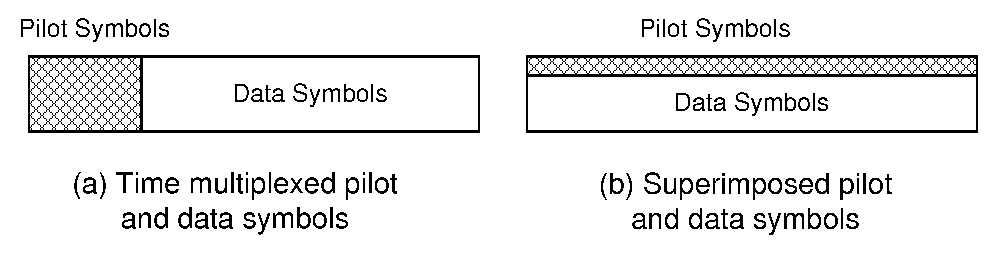
\includegraphics[width=3in, angle=0]{Pilot_Patterns.eps}
\caption{Pilot patterns for channel
estimation.}\label{pilot_pattern} }
\end{figure}

\begin{lemma}\label{Lemma_CRLB}(Cramer-Rao Lower Bound) For the time-multiplexed pilot and data design shown in Fig.~\ref{pilot_pattern}(a) and defined by
\begin{equation}
\begin{array}{rcl}
s_{k}\left(l\right)&=&
\begin{cases}
s_{pk}(l) & 1 \leq l \leq Q \\
s_{dk}(l-Q) & Q+1\leq l\leq L
\end{cases}
\end{array},\label{TMP_k}
\end{equation}
\noindent the CRLB of channel estimation is
\begin{equation}\hspace{-0.3in}
\begin{array}{rcccl}
\sigma_{\mbox{\tiny FL}}^{2}&\geq&\sigma_{\mbox{\tiny
TMP}}^{2}&=&\left[\rho_{h}^2+Q\rho_{p}^2+\left(L-Q\right)\rho_{d}^2\right]^{-1}
\end{array}.\label{CRLB_TMP}
\end{equation}
\noindent For the superimposed pilot and data design shown in
Fig.~\ref{pilot_pattern}(b) and defined by
\begin{equation}
\begin{array}{rcl}
s_{k}\left(l\right)&=&\frac{\sigma_{p}}{P}s_{pk}\left(l\right)+\frac{\sigma_{d}}{P}s_{dk}\left(l\right)\
,\ 1\leq l\leq L\ ,
\end{array}\label{SIP_k}
\end{equation}
\noindent with $\sigma_{p}^2+\sigma_{d}^2=P$, the CRLB of channel
estimation is
\begin{equation}\
\begin{array}{rcccl}
\sigma_{\mbox{\tiny FL}}^{2}&\geq&\sigma_{\mbox{\tiny
SIP}}^{2}&=&\left[\rho_{h}^2+L\left(\rho_{p}^2+\rho_{d}^2\right)\right]^{-1}
\end{array}\label{CRLB_SIP}
\end{equation}
\noindent where $\rho_{p}^2=\frac{\sigma_{p}^2}{\sigma_{n}^2}$
denotes the SNR of received pilot signals and
$\rho_{d}^2=\frac{\sigma_{d}^2}{\sigma_{n}^2}$ denotes the SNR of
received data signals.
\end{lemma}

On the other hand, when $\frac{1}{M}D_{\bh}$ is small enough, the
role of channel quantization becomes important. The squared error
rate distortion $D_{\bh}$ can also be written by
\begin{equation}%\hspace{-0.20in}
\begin{array}{rcl}
D_{\bh}&=&\max\limits_{i}\left\|\bh_{i}-w_{r}{\bw}_{\phi}\right\|_{2}^{2}
\end{array}\label{D_h}
\end{equation}
\noindent with $w_{r}$ denoting the quantized channel amplitude
and ${\bw}_{\phi}$ denoting the quantized channel phase. In
existing MIMO beamforming system design, the receiver usually
tracks the channel amplitude information for adaptive modulation
purpose and phase quantization instead of quantizing and feeding
back the channel amplitude information. In this case, (\ref{D_h})
can be rewritten by
\begin{equation}\hspace{-0.10in}
\begin{array}{rcl}
D_{\bh}&=&\max\limits_{i}\mbox{E}\left\|\bh_{i}-\hat{r}{\bw}_{\phi}\right\|_{2}^{2}\\
&=&\max\limits_{i}\left\{\mbox{E}\left\|r\left(\bv_{i}-{\bw}_{\phi}\right)\right\|_{2}^{2}+\mbox{E}\left\|\delta_{r}{\bw}_{\phi}\right\|_{2}^{2}\right\}\\
&=&M\sigma_{h}^{2}D_{\phi}+\sigma_{\mbox{\tiny FL}}^{2}\ .
\end{array}\label{D_h2}
\end{equation}
\noindent with $\hat{r}$ denoting the channel amplitude estimate.
Therefore a lower bound for distortion rate of channel
quantization for beamforming is

\begin{equation}\hspace{-0.10in}
\begin{array}{rcl}
R(D_{\phi})&=&\min\limits_{E\|\bv_{i}-\hat{\bv}_{i}\|_{2}^{2}\leq
D_{\phi}} I\left(\bv_{i};\
\hat{\bv}_{i}\right)\\
&\geq&\frac{M}{2}\log_{2}\left(\frac{\sigma_{h}^{2}}{(1+\frac{1}{M})\sigma_{\mbox{\tiny
FL}}^{2}+\sigma_{h}^{2}D_{\phi}}\right)\ .
\end{array}\label{R_D_phi}
\end{equation}
\noindent for each beamforming. With the feedback rate of $R$,
(\ref{R_D_phi}) also tells us that the minimum precoding mismatch
for forwardlink MIMO beamforming is
\begin{equation}%\hspace{-0.10in}
\begin{array}{rcl}
D_{\phi}&=&\max\mbox{E}\left\|\hat{\bv}-\bv\right\|_{2}^{2}\\
 &\geq&4^{-\frac{R}{M}}-\left(1+\frac{1}{M}\right)\frac{\sigma_{\mbox{\tiny
FL}}^{2}}{\sigma_{h}^{2}}\ .
\end{array}\label{D_phi}
\end{equation}

\subsection{Bemaforming Mismatch Upper Bound}
\begin{figure}
\center{
\includegraphics[width=3.20in, angle=0]{Voronoi_Bounds2.eps}
\caption{Voronoi cell and various bounds}\label{Voronoi_bound} }
\end{figure}
The beamforming mismatch upper bound mostly depends on the
codebook design. The maximum beamforming mismatch is the largest
radius of the codebook Voronoi cell $\left\{\bcV_{i}:\ 1\leq i\leq
2^{R}\right\}$, which in general is the solution to the
disk-covering problem that still is open. Instead of finding the
exact boundary for the Voronoi cell $\bcV_{i}$, we suggest a
heuristic approach using sphere-packing bound and sphere cap to
approximate the actual polytope boundary. It also is an
approximate of the sphere packing solution, in which all spheres
are supposed to be non-overlappedly placed. With our approach,
sphere caps are overlapped with each other in space but the
interior of them has the same area as the Voronoi cell. The border
of this sphere cap is termed sphere-packing boundary. The
relationship between sphere-packing boundary and Voronoi cell is
shown in Fig.~\ref{Voronoi_bound}. For an uniform random codebook
of size $2^{R}$ in $M$-dimensional Euclid space, the area of a
Voronoi cell is given by
\begin{equation}
\begin{array}{rcl}
A\left(\bcV_{k}\right)&=&
\frac{2{\pi}^{M}}{2^{R}\Gamma\left(M\right)}
\end{array}\label{V_area}
\end{equation}
\noindent where $\Gamma\left(\ast\right)$ denotes the gamma
function. On the other hand, the area of $(m-1)$-complex sphere
cap $\bcC_{m}^{\rm c}\left(\psi,\ R\right)$ with contact angle
$\psi$ and radius $r$ is
\begin{equation}%\hspace{-0.22in}
\begin{array}{l}
A\left(\bcC_{m}^{\rm c}\left(\psi,\
r\right)\right)=\left[1-\cos^{2(m-1)}\left(\psi\right)\right]S_{m}^{\rm
c}\left(r\right),
\end{array}
\end{equation}
\noindent where ${\bcS}_{m}^{\rm c}\left(r\right)$ denotes a
$M$-dimension complex ball in Euclid space with the radius $r$.
The relationship between ${\bcS}_{m}^{\rm c}\left(r\right)$ and
$\bcC_{m}^{\rm c}\left(\psi,\ r\right)$ can be shown in
Fig.~\ref{Voronoi_bound} and it can be verified that
\begin{equation}
\begin{array}{rcl}
A\left(S_{m}^{c}\left(r\right)\right)&=&A\left(\bcC_{m}^{\rm
c}\left(\pi,\ r\right)\right)
\end{array}.
\end{equation}
\noindent With matching the sum area of the sphere-cap with the
whole sphere area, the boundary of a Voronoi cell can be
approximated by a hypershpere or a closed space curve defined in
the following proposition.
\begin{lemma}\label{approx_bound}(Sphere-packing Boundary) The boundary of the uniform complex Voronoi cell $\bcV_{k}$ can be
approximated by a $(M-1)$-unit complex sphere or a closed complex
space curve.
\begin{equation}\hspace{-0.05in}
\begin{array}{rcl}
\bB\left(\bcV_{k}\right)&\approx& \bcS_{M}^{\rm c}(1)\bigcap \bcL_{M}^{\rm c}(\bw_{k},\ \cos(\theta)) \\
&=&\left\{\bv:\ \left\|\bv\right\|=1,\ \angle\left(\bv,\
\bw_{k}\right)=\theta\right\}\ ,
\end{array}
\end{equation}
\noindent where $\bcL_{M}^{\rm c}\left(\bw_{k},\
\cos(\theta)\right)=\left\{\bv:\ \bv^{\rm
H}\bw_{k}=\cos(\theta)\right\}$ denotes a complex space curve and
$\theta$ is
\begin{equation}%\hspace{-0.00in}
\begin{array}{rcl}
\theta&=&\arccos\left(\alpha_{0}\right)
\end{array}
\end{equation}
\noindent with
\begin{equation}\hspace{-0.00in}
\begin{array}{rcl}
\alpha_{0}&=&\left(\frac{2^{R}-1}{2^R}\right)^{\frac{1}{2M-2}}
\end{array}.
\end{equation}
\end{lemma}
With Lemma \ref{approx_bound}, a heuristic upper bound of MIMO
beamforming mismatch is given by

\begin{equation}
\begin{array}{rcl}
D_{\phi}&\leq&1-\left(\frac{2^{R}-1}{2^R}\right)^{\frac{1}{2M-2}}
\end{array}.
\end{equation}


\section{MIMO Feedback Channel Reliability}

The reverselink channel model is a concatenation of a Gaussian
channel and binary erasure channel, which are independent to each
other. When the erasure rate $\varepsilon_{r}$ is high, the
feedback channel reliability is dominated by channel fading, which
means
\begin{equation}%\hspace{-0.00in}
\begin{array}{rcl}
\epsilon\left(R\right)&\approx&\ln\varepsilon_{r}
\end{array}.
\end{equation}
Higher erasure rate on the reverslink feedback channel means it
takes the forwardlink transmitter longer time to accurately filter
out a proper forwardlink precoding word. This also means higher
MIMO precoding mismatch given a certain channel coherent time.
When the erasure rate is low, the reliability of feedback channel
is mostly decided by the additive Gaussian channel noise. In this
case, the well-known sphere-packing upper bound of Gaussian
channel reliability function is
\begin{equation}%\hspace{-0.00in}
\begin{array}{rcl}
\epsilon\left(R\right)&\leq&\epsilon_{\rm sp}\left(R\right)
\end{array}\label{reliability_upper_bound}
\end{equation}
\noindent with $\epsilon_{\rm
sp}\left(R\right)=\frac{\gamma_{\mbox{\tiny
RL}}}{2}-\frac{\sqrt{\gamma_{\mbox{\tiny
RL}}}\eta\cos\theta}{2}-\ln\left(\eta\sin\theta\right)$ and the
lower bound is
\begin{equation}\hspace{-0.30in}
\begin{array}{l}
\epsilon\left(R\right)\geq\begin{cases} \frac{\gamma_{\mbox{\tiny
RL}}}{4}\left(1-\cos\theta\right) &
0\leq R\leq R_{1} \\
\frac{\gamma_{\mbox{\tiny RL}}}{4}\left(1-\cos\theta_{1}\right)
+R_{1}-R_{0}&
R_{1}\leq R\leq R_{2} \\
\epsilon_{\rm sp}\left(R\right) &R_{2}\leq R\leq C
\end{cases}
\end{array}\label{reliability_lower_bound}
\end{equation}
\noindent where $\gamma_{\mbox{\tiny RL}}=\frac{P_{\mbox{\tiny
RL}}}{\sigma^2_{\mbox{\tiny RL}}}$ denotes the reverselink SNR,
$\theta=\arcsin e^{-R}$ denotes the sphere-packing angle,
\begin{equation}\hspace{-0.0in}
\begin{array}{rcl}
\eta&=&\frac{1}{2}\left(\sqrt{\gamma_{\mbox{\tiny
RL}}}\cos\theta+\sqrt{\gamma_{\mbox{\tiny
RL}}\cos^2\theta+4}\right)
\end{array},
\end{equation}
\begin{equation}\hspace{-0.0in}
\begin{array}{rcl}
R_{1}&=&\frac{1}{2}\ln\left(\frac{1}{2}+\frac{1}{2}\sqrt{1+\frac{\gamma_{\mbox{\tiny
RL}}}{4}}\right)
\end{array},
\end{equation}
\begin{equation}\hspace{-0.0in}
\begin{array}{rcl}
R_{2}&=&\frac{1}{2}\ln\left(\frac{1}{2}+\frac{\gamma_{\mbox{\tiny
RL}}}{4}+\frac{1}{2}\sqrt{1+\frac{\gamma_{\mbox{\tiny
RL}}}{4}}\right)
\end{array}
\end{equation}
\noindent and $\theta_{1}=\arcsin e^{-R_{1}}$.

The upper bound and the lower bound of the reliability function in
(\ref{reliability_upper_bound}) and
(\ref{reliability_lower_bound}) are for the case in which there is
no channel estimation error or quantization error in the
forwardlink. On the other hand, the lower bound for channel
estimation is given in Lemma \ref{Lemma_CRLB} and, with the
assumption of uniform random codebook and MIMO channels, the
standard deviation of codebook quantization errors can be found in
the following lemma.
\begin{lemma} The standard deviation
of $\alpha$ is given by
\begin{equation}\hspace{-0.2in}
\begin{array}{rcccl}
\sigma_{\alpha}^2&=&\mbox{E}\left\{\alpha^2\right\}&=&\frac{1}{M}+\frac{M-1}{M}\left(\frac{2^B-1}{2^B}\right)^{\frac{1}{M-1}}
\end{array}.\label{sigma_alpha}
\end{equation}
\end{lemma}

\section{Conclusions}
In this paper, a sphere-packing boundary for codebook Voronoi
decomposition and the beamforming SINR with finite-rate feedback
are formulated. And the effects of imperfect channel estimation
with time-multiplexed pilot pattern or superimposed pilot pattern
on MIMO beamforming are discussed. Finally the scalability and the
tradeoffs in increasing MIMO relay network throughput with
imperfect channel estimation and quantization are discussed.

\small
\bibliographystyle{unsrt}
\bibliography{Cooperative_Relay}
\end{document}
